\chapter[Background]{Background}
\label{Chap:Background}

% No Cites
\nocite{Giplin2023}

\section{Network Stacks}
A network stack, also known as a protocol stack, is a set of protocols that allow communication between devices on a network, regardless of underlying architecture. The most common network stack is the TCP/IP model \cite{Forouzan2021}.

\begin{figure}[h]
    \begin{center}
    \caption{TCP/IP Model of Two Devices and Two Intermediary Nodes \cite{Forouzan2021}}
    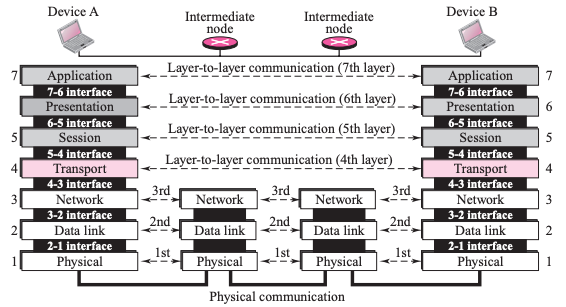
\includegraphics[width=.8\textwidth]{./Figures/TCP_IP_Model.png}
    \label{Fig:3}
    \end{center}
\end{figure}

In FPGA-based projects, the TCP/IP stack can be implemented using a combination of hardware and software components \cite{Perrig2004}. The hardware components, such as the Ethernet MAC and packet processing accelerators, can be designed to handle low-level tasks and offload computationally intensive operations from the software, while the software components, running on the softcore processor, can handle higher-level protocol processing and application-specific tasks \cite{Perrig2004}.

\subsubsection{Ethernet MAC}
The Ethernet Media Access Control (MAC) sublayer, controls access to the shared medium, i.e. switch, in an ethernet-based network \cite{KuroseRoss2021}. In this project, the softcore processor will include an Ethernet MAC module to facilitate communication with other devices on the local area network, such as the switch and connected devices. The MAC module encapsulates higher-layer data into Ethernet frames, transmits them over the physical medium, receives incoming frames, and extracts the data for processing by higher layers \cite{KuroseRoss2021}, the exact buffer format for this can be seen in \ref{Fig:4}.

\begin{figure}[h]
    \begin{center}
    \caption{The Common Ethernet Frame Format, Type II Frame Buffer \cite{Wikipedia_2024}}
    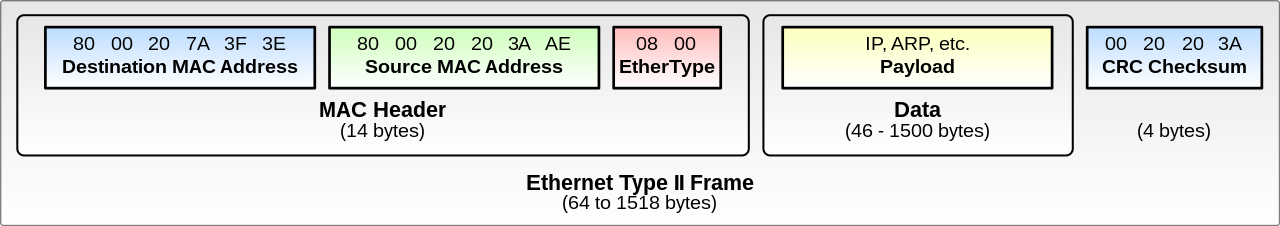
\includegraphics[width=1.0\textwidth]{./Figures/Ethernet_Type_II_Frame_format.png}
    \label{Fig:4}
    \end{center}
\end{figure}

The Ethernet MAC module also features "Carrier Sense Multiple Access with Collision Detection", (CSMA/CD), which manages access to the shared medium and resolves collisions when multiple devices attempt to transmit simultaneously \cite{KuroseRoss2021}. By incorporating an Ethernet MAC module, the processor will be easier to integrate into existing networks.

\subsection{Network Security Methods}
\label{subsection:Network Security Methods}
Network security methods are techniques used to emphasise integrity, confidentiality, and availability of data transmitted over a network. A common method of enhancing network security is encryption, which will be implemented in this project via a  cryptographic acceleration SoC.

\subsubsection{AES Engine and Cryptographic Acceleration}
Cryptographic acceleration is the use of hardware to perform encryption and decryption operations, offloading these computationally intensive tasks from the main processor. To achieve this in the project, the AES Engine SoC by CAST will be implemented. Figure \ref{Fig:5} shows the basic control flow and methodology of the SoC.

\begin{figure}[h]
    \begin{center}
    \caption{AES Engine Block Diagram \cite{CASTInc2024}}
    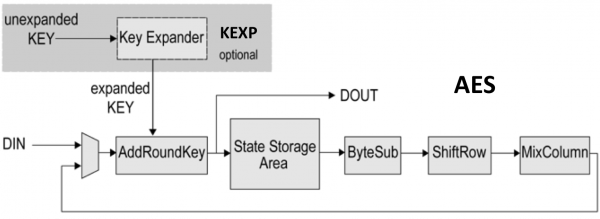
\includegraphics[width=0.9\textwidth]{./Figures/aes-block_0.png}
    \label{Fig:5}
    \end{center}
\end{figure}

The AES core is fully synchronous to data in/data out transmissions, and customisable to several encryption key lengths, and . Most notably, it is implementable via LiteX, see \ref{subsection:VexRiscv}. Using hardware acceleration this way can significantly improve the performance and energy efficiency of cryptographic operations, especially compared to software-based implementations \cite{Stallings2019}.

\section{Operating Systems}
An operating system (OS) is a software that manages computer hardware, software resources, and provides common services for computer programs. This project will explore two different types of operating system design. Real-time operating systems (in this case, Zephyr), and containerised Debian images managed by Kubernetes. 

\subsection{Zephyr (RTOSs)}
A real-time operating system (RTOS) is an OS designed to support real-time applications, which require deterministic and timely processing of data. RTOSs are commonly used in IoT devices due to their ability to grant safe, multi-threaded capabilities to processors as opposed to basic cyclic executive code execution. Additionally, they only consist of the absolute minimum requirements for running on bare-metal hardware.

While there are numerous choices for embedded operating systems, Zephyr is one such RTOS that has had continual open-source support and comes packaged with all the services the project requires. This includes thread management primitives, multicore support and networking \cite{ZephyrProject}.

\subsection{Kubernetes Clusters}
Kubernetes is an open-source container orchestration platform that automates the deployment, scaling, and management of containerized applications. Kubernetes clusters are a set of \textit{nodes} (physical or virtual machines) that run containerized OS images managed by Kubernetes \cite{Burns2019}. With regards to the project, these containers will only need to be capable of networking interfacing and interaction, thus Debian-based images will be more than sufficient.

\section{Field Programmable Gate Arrays (FPGAs)}
FPGAs are integrated circuits that can be programmed to implement custom hardware designs. FPGAs offer flexibility, reconfigurability, and hardware acceleration, making them attractive for implementing custom processors and accelerators for specific applications \cite{Trimberger2018}, such as our network security module.

FPGA devices have inherent resource constraints that must be adhered to. These constraints include the available logic resources (e.g., lookup tables, flip-flops), memory (e.g., block RAM, distributed RAM), and specialized resources (e.g., DSP slices, clock management tiles) \cite{Kuon2008}. This often involves making trade-offs between the number of CPU cores, cache sizes, peripheral support, and the allocation of resources for each portion of hardware \cite{Kuon2008}\cite{Koch2016}.

\subsection{Chosen CPU Model: VexRiscv}
\label{subsection:VexRiscv}
The VexRiscv CPU, a 32-bit RISC-V soft processor core, has been chosen due to its open-source nature, flexibility, and compatibility with the Zephyr RTOS and the LiteX SoC builder framework. VexRiscv is specifically designed for FPGA implementations, meaning that it is conformant to the architectural characteristics of FPGAs, promising a performant and resource-efficient processor system \cite{VexRiscvGitHub}.

Zephyr officially supports the RISC-V architecture, and VexRiscv has been successfully integrated with Zephyr in various projects \cite{ZephyrProject}. Moreover, VexRiscv is compatible with LiteX, an open-source SoC builder framework that simplifies the integration of processor cores, peripherals, and custom hardware modules \cite{LiteXProject}. LiteX provides a high-level framework for generating and configuring SoC designs, making it easier to integrate VexRiscv into a complete system \cite{LiteXProject}. This compatibility is proven by well-documented examples and guides available in the Zephyr and LiteX communities \cite{ZephyrProject}\cite{LiteXProject}.Compared to other typical CPU models, such as ARM Cortex-M, Xilinx MicroBlaze, or Intel NIOS II, VexRiscv also has the advantages of being open-source. This lack of IP protection enables the addition of custom instructions and extensions tailored to the specific requirements \cite{VexRiscvGitHub}, allowing the project to take full advantage of the Arty S7 Board.

The Arty S7 board features a Xilinx Spartan-7 FPGA (XC7S50), which offers a moderate amount of logic resources (52,160 logic cells) and memory (2,700 Kb), with a universal clock rate of 100MHz \cite{Arty_S7_Schematic}. VexRiscv's resource-efficient design makes it a viable option for the Arty S7 board. By configuring VexRiscv with appropriate options, such as a balanced pipeline, moderate cache sizes, and essential peripherals, it is possible to implement a dual-core system that fits within the FPGA's constraints while leaving room for additional modules, such as the ethernet MAC or AES engine.

Lastly, VexRiscv benefits from ongoing community support. The availability of open-source tools, such as SpinalHDL, LiteX, and SBT (Scala Build Tool), form the basis for a complete development environment \cite{LiteXProject} \cite{SpinalHDL}.